\documentclass[12pt,a4paper]{article}

% =========================
% Pacotes básicos
% =========================
\usepackage[utf8]{inputenc}
\usepackage[T1]{fontenc}
\usepackage[brazil]{babel}
\usepackage{graphicx}           % Inclusão de imagens
\usepackage{float}              % Controle de posição de figuras/tabelas
\usepackage{amsmath, amssymb}   % Símbolos matemáticos
\usepackage{caption}            % Legendas personalizadas
\usepackage{cite}               % Gerenciamento de citações
\usepackage{listings}           % Blocos de código (listings)
\usepackage{enumitem}           % Listas
\usepackage{xcolor}             % Cores no listings

% Algoritmos: usar algorithm + algpseudocode (substitui o antigo 'algorithmic')
\usepackage{algorithm}
\usepackage{algpseudocode}

\usepackage[hidelinks]{hyperref}
\usepackage{bookmark}

% =========================
% Configurações
% =========================
\lstset{
  language=Python,
  basicstyle=\ttfamily\small,
  numbers=left,
  numberstyle=\tiny,
  frame=single,
  breaklines=true,
  keywordstyle=\color{blue}\bfseries,
  stringstyle=\color{red},
  commentstyle=\color{green!60!black}\itshape,
  showstringspaces=false
}

\graphicspath{{./img/}} % Diretório das imagens

% Opção: deixar comentários do algpseudocode alinhados à direita
\algrenewcommand\algorithmiccomment[1]{\hfill\(\triangleright\)~#1}

% =========================
\begin{document}
% =========================

% =========================
% CAPA
% =========================
\begin{titlepage}
    \centering
    {\Large \textbf{Universidade Federal de Minas Gerais}}\\[0.3cm]
    {\large Engenharia de Sistemas}\\[2cm]
    
    {\Huge \textbf{Relatório do Trabalho Prático II - Coloração em Grafos}}\\[1.5cm]
    
    \textbf{Fundamentos de Inteligência Artificial}\\[0.5cm]
    \textbf{Professores:} Cristiano Castro e João Pedro Campos\\[1.5cm]
    
    \begin{flushleft}
        \textbf{Alunos:}\\
        Áquila Oliveira Souza --- 2021019327\\
        Arthur Jorge --- 2022055718\\
        Felippe Veloso Marinho --- 2021072260\\
        Jefferson Pereira de Souza --- 2022099049\\
        Josoé Santos Queiroz --- 2019026982
    \end{flushleft}
    
    \vfill
    {\large Belo Horizonte, MG}\\
    {\large \today}
\end{titlepage}

\clearpage
\pdfbookmark[1]{Sumário}{toc}
\tableofcontents
\clearpage

% =========================
% INTRODUÇÃO
% =========================
\section{Introdução}
A coloração de grafos é um problema clássico da teoria dos grafos com diversas aplicações práticas, como na alocação de frequências em redes sem fio, escalonamento de tarefas e planejamento de horários. O objetivo é atribuir cores aos vértices de um grafo de forma que vértices adjacentes não compartilhem a mesma cor, minimizando o número total de cores utilizadas.

Neste relatório, apresentamos uma solução para o problema de coloração de grafos, modelando-o formalmente como um grafo em que as arestas representam restrições binárias entre os vértices.

Além disso, detalhamos as heurísticas utilizadas para resolver o problema, discutindo suas abordagens teóricas e implementações práticas. Também analisamos as decisões tomadas durante o desenvolvimento e os resultados obtidos.

O documento está organizado da seguinte forma: na Seção 2, apresentamos o problema de coloração de grafos; na Seção 3, discutimos as heurísticas teóricas; na Seção 4, detalhamos suas implementações; e, por fim, na Seção 5, apresentamos as conclusões e possíveis melhorias futuras.

\section{Problema da Coloração de Grafos}
\label{sec:problema}
O problema da coloração de grafos consiste em associar uma cor a cada vértice de um grafo \( G = (V, E) \), de modo que dois vértices adjacentes \( u, v \in V \) não possuam a mesma cor. O desafio é minimizar o número total de cores utilizadas, conhecido como número cromático do grafo. Trata-se de um problema NP-difícil, o que motiva o uso de heurísticas e metaheurísticas para obtenção de soluções aproximadas em tempo viável.

\section{Heurísticas — Fundamentação Teórica}
\label{sec:heuristicas}

\subsection{Random Walk (RW)}
O \textit{Random Walk} é uma heurística de busca estocástica que explora o espaço de soluções movendo-se aleatoriamente entre colorações possíveis. O processo inicia-se com uma coloração aleatória e, em seguida, ajusta-se gradualmente os conflitos — isto é, os casos em que vértices adjacentes possuem a mesma cor. Esse procedimento é repetido até que se encontre uma solução viável ou que seja atingido um critério de parada.

\subsection{Best Improvement (BI)}
O \textit{Best Improvement}, por ser heurística de busca local que busca a "melhor melhoria" possível em cada iteração, inicia-se de uma solução inicial, depois o algoritmo avalia todas as alterações viáveis e seleciona aquela que proporciona o maior ganho.
No contexto da coloração de grafos, o objetivo é reduzir o número de conflitos (vértices adjacentes com a mesma cor) ou diminuir o total de cores utilizadas. 

\subsection{First Improvement with Random Local Search (FI-RS)}
O \textit{First Improvement with Random Local Search} (FI-RS) é uma metaheurística de busca local que combina o \textit{Random Local Search} e o \textit{First Improvement}.  
O primeiro realiza pequenas alterações aleatórias em uma solução, enquanto o segundo aceita a primeira melhoria encontrada, sem necessidade de examinar todas as opções.  
Aplicado à coloração de grafos, o FI-RS busca uma coloração com o menor número de conflitos de forma eficiente, evitando uma exploração exaustiva do espaço de busca.

\subsection{First Improvement with Any Conflict (FI-AC)}
A partir de uma solução inicial, possivelmente com conflitos, o algoritmo tenta melhorá-la iterativamente.  
A estratégia \textit{First Improvement} implica aceitar imediatamente o primeiro movimento que melhora a solução, sem buscar o melhor global. Já o termo \textit{Any Conflict} indica que qualquer vértice envolvido em conflito pode ser escolhido aleatoriamente para modificação.  
No problema de coloração de grafos, o FI-AC aprimora progressivamente a coloração até eliminar os conflitos entre vértices adjacentes.

\subsection{Simulated Annealing (SA)}
O \textit{Simulated Annealing} (SA) é uma metaheurística de busca estocástica inspirada no processo físico de recozimento térmico de metais. Nesse processo, o material é aquecido e resfriado lentamente para alcançar uma configuração estável de mínima energia.  
Analogamente, o SA aceita piores soluções no início (alta temperatura) e torna-se mais seletivo à medida que a “temperatura” diminui, buscando escapar de ótimos locais e aproximar-se de uma solução globalmente ótima.  
Na coloração de grafos, o SA visa reduzir gradualmente os conflitos de coloração, aceitando ocasionalmente soluções piores para explorar melhor o espaço de busca.

\subsection{Algoritmo Genético (GA)}
O \textit{Algoritmo Genético} (GA) é uma metaheurística inspirada nos princípios da evolução natural, proposta originalmente por Holland (1975). Ele baseia-se em mecanismos biológicos como seleção, cruzamento e mutação para evoluir uma população de soluções ao longo das gerações.

No contexto do problema de coloração de grafos, cada indivíduo da população representa uma coloração possível, onde os genes correspondem às cores atribuídas aos vértices. O processo evolutivo busca minimizar o número de conflitos e reduzir o total de cores utilizadas.

Os Algoritmos Genéticos (AG) são técnicas de otimização inspiradas no processo de seleção natural. Eles trabalham com uma população de soluções candidatas, que evoluem ao longo do tempo através de operadores genéticos como seleção, cruzamento (crossover) e mutação.

\section{Heurísticas - Implementação}

\subsection{Random Walk (RW)}
Por ser uma heurística de busca estocástica que explora o espaço de soluções movendo-se aleatoriamente entre as colorações possíveis, o processo se inicia com uma coloração aleatória e, em seguida, ajusta-se gradualmente os conflitos. Esse procedimento se repete até que não existam mais conflitos (uma coloração válida) ou que o limite de iterações seja atingido.
\begin{algorithm}[H]
\caption{Random Walk (RW)}
\label{alg:random_walk}
\begin{algorithmic}[1]
\Require Grafo \(G\), Coloração inicial \(C_{\text{inicial}}\), Conjunto de cores \(\mathcal{K}\), Máx. iterações \(I_{\max}\)
\Ensure Coloração \(C\) com o menor número de conflitos
\State \(C \gets C_{\text{inicial}}\)
\State \(conflitos \gets \text{ContarConflitos}(G, C)\)
\For{\(i = 1\) to \(I_{\max}\)}
    \State \(v \gets \text{EscolherAleatoriamente}(\text{Vértices}(G))\)
    \State \(k_{\text{novo}} \gets \text{EscolherAleatoriamente}(\mathcal{K})\)
    \State \(C_{\text{novo}} \gets C\)
    \State \(C_{\text{novo}}[v] \gets k_{\text{novo}}\)
    \State \(conflitos_{\text{novo}} \gets \text{ContarConflitos}(G, C_{\text{novo}})\)
    \If{\(conflitos_{\text{novo}} < conflitos\)}
        \State \(C \gets C_{\text{novo}}\)
        \State \(conflitos \gets conflitos_{\text{novo}}\)
        \If{\(conflitos = 0\)} \State \textbf{break} \EndIf
    \EndIf
\EndFor
\State \Return \(C, conflitos\)
\end{algorithmic}
\end{algorithm}

\subsection{Best Improvement (BI)}
O \textit{Best Improvement} é uma heurística de busca local que busca a melhor melhoria possível em cada iteração. A partir de uma solução inicial, o algoritmo avalia todas as alterações viáveis dentro de uma vizinhança definida e seleciona aquela que proporciona o maior ganho. Como o objetivo é reduzir o número de conflitos (vértices adjacentes com a mesma cor), iteramos através de uma busca exaustiva nos dois loops verificando se há uma nova coloração com menos conflitos até que não haja mais.
\begin{algorithm}[H]
\caption{Best Improvement (BI)}
\label{alg:best_improvement}
\begin{algorithmic}[1]
\Require Grafo \(G\), Coloração inicial \(C_{\text{inicial}}\), Conjunto de cores \(\mathcal{K}\), Máx. iterações \(I_{\max}\)
\Ensure Coloração \(C\) com o menor número de conflitos
\State \(C \gets C_{\text{inicial}}\)
\State \(conflitos \gets \text{ContarConflitos}(G, C)\)
\For{\(i = 1\) to \(I_{\max}\)}
    \State \(C_{\text{melhor}} \gets C\)
    \State \(melhor\_melhora \gets 0\)
    \ForAll{vértices \(v \in \text{Vértices}(G)\)}
        \ForAll{cores \(k \in \mathcal{K}\)}
            \State \(C_{\text{temp}} \gets C\)
            \State \(C_{\text{temp}}[v] \gets k\)
            \State \(conflitos_{\text{temp}} \gets \text{ContarConflitos}(G, C_{\text{temp}})\)
            \State \(melhora \gets conflitos - conflitos_{\text{temp}}\)
            \If{\(melhora > melhor\_melhora\)}
                \State \(melhor\_melhora \gets melhora\)
                \State \(C_{\text{melhor}} \gets C_{\text{temp}}\)
            \EndIf
        \EndFor
    \EndFor
    \If{\(melhor\_melhora = 0\)} \State \textbf{break} \Comment{Ótimo local} \EndIf
    \State \(C \gets C_{\text{melhor}}\)
    \State \(conflitos \gets conflitos - melhor\_melhora\)
    \If{\(conflitos = 0\)} \State \textbf{break} \EndIf
\EndFor
\State \Return \(C, conflitos\)
\end{algorithmic}
\end{algorithm}

\subsection{First Improvement with Random Local Search (FI-RS)}
O \textit{First Improvement with Random Local Search} (FI-RS) é uma metaheurística de busca local que combina o \textit{Random Local Search} e o \textit{First Improvement}. O algoritmo seleciona aleatoriamente um vértice e atribui-lhe uma cor aleatória. Este novo estado é então avaliado. O movimento é aceito se a nova coloração for estritamente melhor (tiver menos conflitos) que a coloração atual, aplicando o critério \textit{First Improvement}.
O código do FI-RS implementa essa lógica iniciando com uma coloração e contando os conflitos. A cada iteração, um vértice e uma nova cor são escolhidos aleatoriamente (\textit{Random Local Search}). Se esta nova coloração resultar em menos conflitos (\textit{First Improvement}), ela é imediatamente aceita e o loop continua. O processo é limitado por um número máximo de iterações.
\begin{algorithm}[H]
\caption{First Improvement with Random Local Search (FI-RS)}
\label{alg:fi_rs}
\begin{algorithmic}[1]
\Require Grafo \(G\), Coloração inicial \(C_{\text{inicial}}\), Conjunto de cores \(\mathcal{K}\), Máx. iterações \(I_{\max}\)
\Ensure Coloração \(C\) com o menor número de conflitos
\State \(C \gets C_{\text{inicial}}\)
\State \(conflitos \gets \text{ContarConflitos}(G, C)\)
\For{\(i = 1\) to \(I_{\max}\)}
    \State \(v \gets \text{EscolherAleatoriamente}(\text{Vértices}(G))\)
    \State \(k_{\text{novo}} \gets \text{EscolherAleatoriamente}(\mathcal{K})\)
    \State \(C_{\text{novo}} \gets C\)
    \State \(C_{\text{novo}}[v] \gets k_{\text{novo}}\)
    \State \(conflitos_{\text{novo}} \gets \text{ContarConflitos}(G, C_{\text{novo}})\)
    \If{\(conflitos_{\text{novo}} < conflitos\)}
        \State \(C \gets C_{\text{novo}}\)
        \State \(conflitos \gets conflitos_{\text{novo}}\)
        \If{\(conflitos = 0\)} \State \textbf{break} \EndIf
    \EndIf
\EndFor
\State \Return \(C, conflitos\)
\end{algorithmic}
\end{algorithm}

\noindent\textit{Nota:} No contexto de coloração de grafos, o FI-RS costuma ficar idêntico ao RW, onde a busca local aleatória é a escolha de \(v\) e \(k_{\text{novo}}\), e o \textit{First Improvement} é o critério \(conflitos_{\text{novo}} < conflitos\).

\subsection{First Improvement with Any Conflict (FI-AC)}
O \textit{First Improvement with Any Conflict} (FI-AC) é uma variação da heurística de busca local. A estratégia \textit{First Improvement} implica aceitar imediatamente o primeiro movimento que melhora a solução, sem buscar o melhor global. Já o termo \textit{Any Conflict} indica que qualquer vértice envolvido em conflito pode ser escolhido aleatoriamente para modificação.
O código do FI-AC reflete essa prioridade de busca, onde a cada iteração, apenas um vértice escolhido aleatoriamente entre os \textit{conflitantes} (\textit{Any Conflict}) é avaliado. O algoritmo testa todas as cores disponíveis para este vértice, aceitando o primeiro movimento que reduz o número total de conflitos (\textit{First Improvement}) e interrompendo a busca interna de cores.
\begin{algorithm}[H]
\caption{First Improvement with Any Conflict (FI-AC)}
\label{alg:fi_ac}
\begin{algorithmic}[1]
\Require Grafo \(G\), Coloração inicial \(C_{\text{inicial}}\), Conjunto de cores \(\mathcal{K}\), Máx. iterações \(I_{\max}\)
\Ensure Coloração \(C\) com o menor número de conflitos
\State \(C \gets C_{\text{inicial}}\)
\State \((conflitos, V_{\text{conflito}}) \gets \text{RetornarConflitos}(G, C)\)
\If{\(conflitos = 0\)} \State \Return \(C, conflitos\) \EndIf
\For{\(i = 1\) to \(I_{\max}\)}
    \State \(v \gets \text{EscolherAleatoriamente}(V_{\text{conflito}})\)
    \ForAll{cores \(k \in \mathcal{K}\)}
        \State \(C_{\text{novo}} \gets C\)
        \State \(C_{\text{novo}}[v] \gets k\)
        \State \((conflitos_{\text{novo}}, V_{\text{novo\_conflito}}) \gets \text{RetornarConflitos}(G, C_{\text{novo}})\)
        \If{\(conflitos_{\text{novo}} < conflitos\)}
            \State \(C \gets C_{\text{novo}}\)
            \State \(conflitos \gets conflitos_{\text{novo}}\)
            \State \(V_{\text{conflito}} \gets V_{\text{novo\_conflito}}\)
            \If{\(conflitos = 0\)} \State \textbf{break} \Comment{Solução encontrada} \EndIf
            \State \textbf{break} \Comment{Aceita a primeira melhoria}
        \EndIf
    \EndFor
    \If{\(conflitos = 0\)} \State \textbf{break} \EndIf
\EndFor
\State \Return \(C, conflitos\)
\end{algorithmic}
\end{algorithm}

\subsection{Simulated Annealing (SA)}
O \textit{Simulated Annealing} (SA) é uma meta-heurística baseada no processo de recozimento de metais, onde a temperatura é lentamente reduzida para permitir que o material atinja um estado de energia mínima. Em problemas de otimização, ele é parecido com o First Improvement, mas aceita soluções piores (com mais conflitos) com uma probabilidade que é função do parâmetro de temperatura (que decai com o tempo) e da diferença entre o número de conflitos entre a coloração atual e a nova coloração. Essa aceitação de passos "ruins" permite que o algoritmo escape de ótimos locais.
O código do SA implementa o mecanismo de recozimento utilizando um parâmetro de temperatura ($T$) que decai a cada iteração. A cada passo, uma mudança de cor é proposta aleatoriamente em um vértice, e a diferença de conflitos ($\Delta E$) é calculada. Se $\Delta E < 0$ (melhoria), a mudança é aceita. Caso contrário (piora), a aceitação é estocástica, determinada por uma função de probabilidade $P$ que depende de $\Delta E$ e da temperatura $T$ atual, garantindo a exploração no início e a explotação no final.
\begin{algorithm}[H]
\caption{Simulated Annealing (SA)}
\label{alg:simulated_annealing}
\begin{algorithmic}[1]
\Require Grafo \(G\), Coloração inicial \(C_{\text{inicial}}\), Conjunto de cores \(\mathcal{K}\), Máx. iterações \(I_{\max}\), Temperatura inicial \(T_0\)
\Ensure Coloração \(C\) com o menor número de conflitos
\State \(C \gets C_{\text{inicial}}\)
\State \(conflitos \gets \text{ContarConflitos}(G, C)\)
\State \(T \gets T_0\)
\For{\(i = 1\) to \(I_{\max}\)}
    \State \(v \gets \text{EscolherAleatoriamente}(\text{Vértices}(G))\)
    \State \(k_{\text{novo}} \gets \text{EscolherAleatoriamente}(\mathcal{K})\)
    \State \(C_{\text{novo}} \gets C\)
    \State \(C_{\text{novo}}[v] \gets k_{\text{novo}}\)
    \State \(conflitos_{\text{novo}} \gets \text{ContarConflitos}(G, C_{\text{novo}})\)
    \State \(\Delta E \gets conflitos_{\text{novo}} - conflitos\) \Comment{Diferença de ``energia''}
    \If{\(\Delta E < 0\)} \Comment{Melhoria}
        \State \(C \gets C_{\text{novo}}\)
        \State \(conflitos \gets conflitos_{\text{novo}}\)
    \Else
        \State \(P \gets \text{ProbabilidadeAceitacao}(\Delta E, T)\)
        \State \textbf{if} \(\text{Aleatorio}(0,1) < P\) \textbf{then}
            \State \hspace{1.5em} \(C \gets C_{\text{novo}}\) \Comment{Aceita piora estocasticamente}
            \State \hspace{1.5em} \(conflitos \gets conflitos_{\text{novo}}\)
        \State \textbf{end if}
    \EndIf
    \If{\(conflitos = 0\)} \State \textbf{break} \EndIf
    \State \(T \gets \text{DecairTemperatura}(T, i)\)
\EndFor
\State \Return \(C, conflitos\)
\end{algorithmic}
\end{algorithm}

\subsection{Algoritmo Genético (GA)}
O \textit{Algoritmo Genético} (GA) é uma meta-heurística de busca global inspirada na evolução biológica. Ele evolui um conjunto de soluções candidatas, denominado população. A cada passo (geração), as soluções atuais interagem entre si através de operadores genéticos (seleção, recombinação (crossover) e mutação) para produzir uma nova população, buscando a convergência para soluções de alta qualidade. No problema de coloração, cada indivíduo (cromossomo) na população representa uma coloração completa do grafo.
O código do GA inicia com a geração de uma população de colorações candidatas. O processo é iterado por um número máximo de gerações, onde a cada ciclo, pares de pais são selecionados. Estes pais geram dois filhos através da recombinação (\textit{crossover}), e uma mutação aleatória é aplicada aos filhos. A nova população substitui a antiga, e a melhor solução encontrada até o momento ($C_{\text{melhor}}$) é atualizada, guiando a evolução para colorações com menos conflitos.
\begin{algorithm}[H]
\caption{Algoritmo Genético (GA) para Coloração}
\label{alg:genetic_algorithm}
\begin{algorithmic}[1]
\Require Grafo \(G\), Conjunto de cores \(\mathcal{K}\), Tamanho da população \(N\), Máx. gerações \(G_{\max}\)
\Ensure Melhor coloração \(C_{\text{melhor}}\)
\State \(\mathcal{P} \gets \text{GerarPopulacaoInicial}(N, G, \mathcal{K})\)
\State \(C_{\text{melhor}} \gets \text{MelhorSolucao}(\mathcal{P})\)
\For{\(g = 1\) to \(G_{\max}\)}
    \State \(\mathcal{P}_{\text{nova}} \gets \emptyset\)
    \For{\(j = 1\) to \(N/2\)}
        \State \(P_1, P_2 \gets \text{Selecao}(\mathcal{P})\) \Comment{Torneio, Roleta, etc.}
        \State \(F_1, F_2 \gets \text{Crossover}(P_1, P_2)\)
        \State \(F_1 \gets \text{Mutacao}(F_1, \mathcal{K})\)
        \State \(F_2 \gets \text{Mutacao}(F_2, \mathcal{K})\)
        \State \(\mathcal{P}_{\text{nova}} \gets \mathcal{P}_{\text{nova}} \cup \{F_1, F_2\}\)
    \EndFor
    \State \(\mathcal{P} \gets \mathcal{P}_{\text{nova}}\)
    \State \(C_{\text{atual\_melhor}} \gets \text{MelhorSolucao}(\mathcal{P})\)
    \If{\(\text{Avaliar}(C_{\text{atual\_melhor}}) < \text{Avaliar}(C_{\text{melhor}})\)}
        \State \(C_{\text{melhor}} \gets C_{\text{atual\_melhor}}\)
    \EndIf
    \If{\(\text{Avaliar}(C_{\text{melhor}}) = 0\)} \State \textbf{break} \EndIf
\EndFor
\State \Return \(C_{\text{melhor}}, \text{Avaliar}(C_{\text{melhor}})\)
\end{algorithmic}
\end{algorithm}

\subsection{DSATUR}
O DSATUR (Degree of Saturation) é uma heurística gulosa para o problema de coloração de grafos que prioriza a coloração dos vértices com maior grau de saturação, ou seja, aqueles que possuem o maior número de cores diferentes já atribuídas aos seus vizinhos. Essa heurística é particularmente eficaz para o problema de coloração., pois ao focar nos vértices mais "constrangidos", ela tende a minimizar o número total de cores necessárias para uma coloração válida.

A implementação do DSATUR envolve os seguintes passos principais:
\begin{itemize}
 \item Os vértices do grafo são ordenados com base em seu grau de saturação.
 \item O vértice mais saturado é selecionado para a coloração.
 \item A cor mais baixa possível é atribuída ao vértice selecionado, garantindo que não haja conflitos com os vizinhos já coloridos.
 \item O processo é repetido até que todos os vértices estejam coloridos.
\end{itemize}

\section{Experimentos}
O objetivo dos experimentos é avaliar o desempenho das heurísticas implementadas na resolução do problema de coloração de grafos. Para isso, realizamos uma série de 30 execuções para cada heurística, utilizando diferentes instâncias do problema. As instâncias seleciondas foram a fornecida no enunciado da tarefa e outras duas instâncias.

Cada execução foi monitorada quanto ao tempo de processamento e a porcentagem de instâncias resolvidas. Neste experimento não limitamos o número de cores mas limitamos o tempo de execução para 2 segundos por execução.

As instâncias utilizadas nos experimentos foram:

\begin{itemize}
 \item \textbf{default}: A instância padrão fornecida no enunciado da tarefa, servindo como base para comparação entre as heurísticas.
 \item \textbf{myciel.5.col}: Uma instância maior com 47 vértices, representando um desafio mediano para as heurísticas.
 \item \textbf{queen9-9.col}: A maior instância utilizada, com 81 vértices e 2112 aréstas, testando a escalabilidade e eficiência das heurísticas em problemas maiores.
\end{itemize}

\begin{figure}[H]
    \centering
    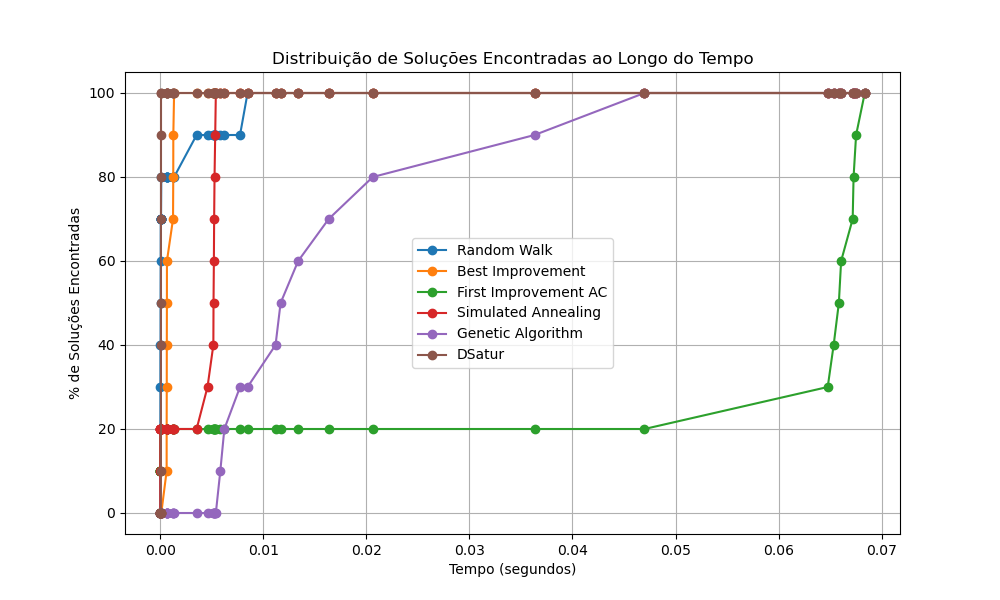
\includegraphics[width=1\textwidth]{./img/output-default.png}
    \caption{Experimento com a instância default.}
    \label{fig:experimento-default}
\end{figure}

Neste experimento, podemos observar que a heurística DSATUR se destacou significativamente, alcançando uma taxa de resolução de 100\% das instância quase instantaneamente, com um tempo médio de execução de apenas 0.01 segundos. Isso indica que o DSATUR é altamente eficiente para a instância default, conseguindo encontrar soluções ótimas rapidamente.

\begin{figure}[H]
    \centering
    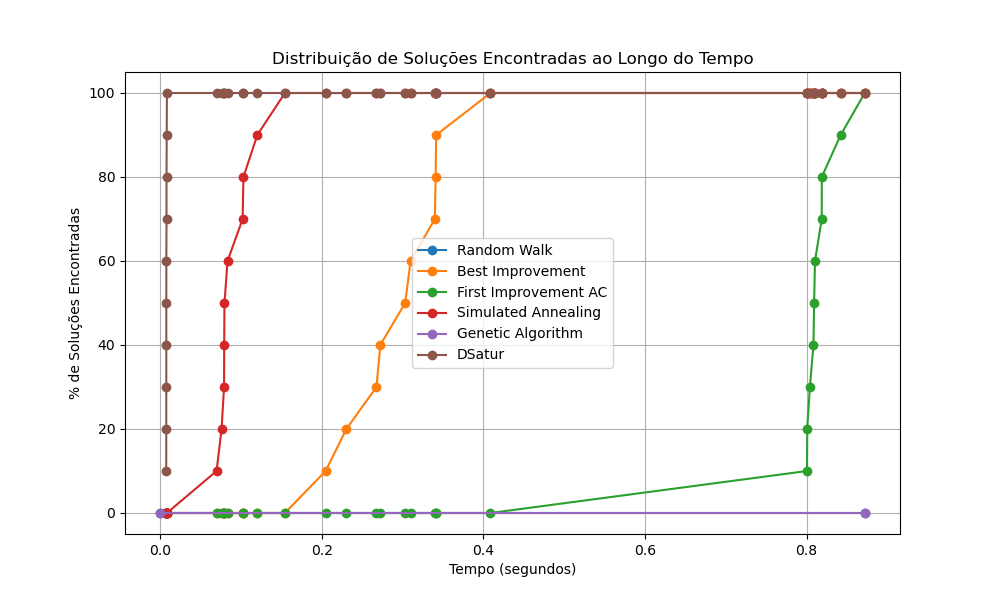
\includegraphics[width=1\textwidth]{./img/output-myciel5.png}
    \caption{Experimento com a instância myciel.5.col.}
    \label{fig:experimento-myciel5}
\end{figure}

\begin{figure}[H]
    \centering
    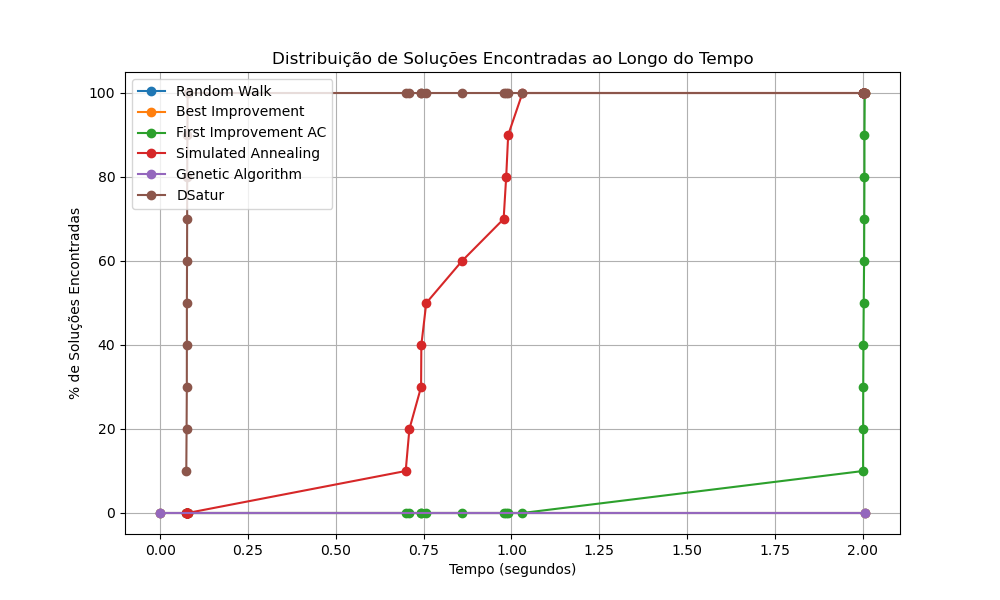
\includegraphics[width=1\textwidth]{./img/output-queen9-9.png}
    \caption{Experimento com a instância queen9-9.col.}
    \label{fig:experimento-queen9-9}
\end{figure}

Nos dois exeperimentos subsequentes, com as instâncias myciel.5.col e queen9-9.col, alguns algorítmos não encontraram soluções viáveis dentro do limite de tempo estabelecido. E por isto não aparecem nos gráficos. Esses resultados ressaltam a importância de considerar a complexidade do problema e a adequação das heurísticas utilizadas para diferentes instâncias.

Nos experimentos com instâncias maiores, como myciel.5.col e queen9-9.col, observamos que a heurística DSATUR continuou a se destacar, mantendo uma taxa de resolução de 100\% em ambas as instâncias. Isso demonstra a robustez e eficiência do DSATUR mesmo em problemas mais complexos.

\section{Conclusão}
O trabalhou explorou o problema NP-difícil da coloração de grafos por meio de implementações de diversas heurísticas de busca local e metaheurísticas como (RW, BI, FI-RS, FI-AC, SA, GA) além da heurística gulosa DSATUR. O objetivo principal foi complementar a implementação dada como referência e analisar a adequação e eficiência dessas abordagens em diferentes instâncias de grafos.

Em relação aos resultados experimentais, a heurística gulosa DSATUR demonstrou ser, de longe, o método mais robusto e eficiente entre os avaliados. Em todas as três instâncias testadas (Default, myciel.5.col e queen9-9.col), o DSATUR atingiu uma taxa de resolução de $100\%$ das execuções, com um tempo médio de execução quase instantâneo (e.g., $0.01$ segundos para a instância \textbf{default}). Este desempenho superior é inerente à natureza gulosa do DSATUR, que toma decisões localmente ótimas (priorizando vértices mais saturados) que tendem a levar rapidamente a uma coloração válida.
Em contraste, as heurísticas de busca local (RW, BI, FI-RS, FI-AC) e as metaheurísticas (SA, GA) enfrentaram dificuldades notáveis nas instâncias maiores (\textbf{myciel.5.col} e \textbf{queen9-9.col}). O fato de "algoritmos não terem encontrado soluções viáveis dentro do limite de tempo" para instâncias de tamanho mediano a grande ressalta o desafio da busca local e global em espaços de solução complexos. Embora essas heurísticas sejam projetadas para otimizar o número de conflitos, sua eficácia é comprometida pelo limite de iterações ou pela dificuldade de escapar de ótimos locais. O desempenho fraco sugere que, para problemas de coloração, a estratégia gulosa de construção (como o DSATUR) é mais eficaz para encontrar rapidamente uma solução válida do que as estratégias de busca e refinamento baseadas na minimização de conflitos.

Futuras melhorias poderiam ser feitas através da integração de uma fase de Busca Local (BI ou FI-AC) após o Algoritmo Genético, utilizando a melhor solução da população como ponto de partida. Outra ideia seria a utilização do DSATUR como método de coloração inicial para todos os algoritmos de busca, fornecendo um ponto de partida de qualidade superior e reduzindo drasticamente o número inicial de conflitos.

\cleardoublepage
\phantomsection
\section*{Referências}
\addcontentsline{toc}{section}{Referências}

\begin{thebibliography}{99}

\bibitem{qehaja2025}
QEHJA, B.; HAJRIZI, E.; ALI, M. A. A Hybrid Graph-Coloring and Metaheuristic Framework for Dynamic Wireless Sensor Networks. \textit{Preprints}, 2025. Disponível em: \url{https://www.preprints.org/manuscript/202507.0720/v1/download}. Acesso em: 26 out. 2025.

\bibitem{bihani2025}
BIHANI, O. A Heuristic for Graph Coloring Based on the Ising Model. \textit{Mathematics}, v. 13, n. 18, p. 2976, 2025. Disponível em: \url{https://www.mdpi.com/2227-7390/13/18/2976}. Acesso em: 26 out. 2025.

\bibitem{yakut2025}
YAKUT, S. A robust and efficient algorithm for graph coloring problem. \textit{Journal of King Saud University - Computer and Information Sciences}, 2025. Disponível em: \url{https://www.sciencedirect.com/science/article/pii/S1110866525000696}. Acesso em: 26 out. 2025.

\bibitem{dokeroglu2025}
DOKEROGLU, T.; BOGAZ, S.; KESKIN, M. An island-parallel ensemble metaheuristic algorithm for graph coloring problems. \textit{arXiv preprint arXiv:2504.15082}, 2025. Disponível em: \url{https://arxiv.org/html/2504.15082v1}. Acesso em: 26 out. 2025.

\end{thebibliography}

\end{document}
